\documentclass[12pt, letterpaper]{article}
\usepackage{graphicx}
\usepackage[margin=1in]{geometry}
\usepackage{amsmath, amssymb, amsthm, mathrsfs}
\usepackage{fancyhdr}
\usepackage{tikz}
\usepackage{enumerate}
\usepackage{cancel}
\usetikzlibrary{positioning, trees, calc}
\usepackage[utf8]{inputenc}
\usepackage{xcolor}
\usepackage{framed}
\usepackage{multirow}
\title{HW 1.3}
\author{Your Name}
\date{\today}
\pagestyle{fancy}
\renewcommand{\headrulewidth}{0pt}
\renewcommand{\footrulewidth}{0pt}
\fancyhf{}
\rhead{
    Zack Abdirashid\\
    4/9/26 \\
    MATH 405
}
\rfoot{Page \thepage}
\begin{document}
\paragraph{\underline{3.3} \\ \\} 
\textbf{5.}\begin{tabular}[t]{l}
    Every month a plastics plant must make batches of five different types of plastic toys. \\
    There is a conversion cost $c_{ij}$ in switching from the production of toy $i$ to toy $j$, shown \\
    in the matrix. Find a sequence of toy production (to be followed for many months) that \\
    minimizes the sum of the monthly conversion costs.
\end{tabular}

\vspace{1.5em}
\begin{center}
\renewcommand{\arraystretch}{1.25}
\setlength{\tabcolsep}{12pt}
\begin{tabular}{@{}ll|ccccc@{}}
\multicolumn{2}{@{}r|}{} & \multicolumn{5}{c@{}}{To} \\[-0.2ex]
\multicolumn{2}{@{}r|}{} & $T_1$ & $T_2$ & $T_3$ & $T_4$ & $T_5$ \\
\cline{3-7}
\multirow{5}{*}[-2pt]{\raisebox{0pt}[0pt][0pt]{From}} & $T_1$ & \textemdash & 3 & 2 & 4 & 3 \\
& $T_2$ & 4 & \textemdash & 4 & 5 & 5 \\
& $T_3$ & 5 & 3 & \textemdash & 4 & 4 \\
& $T_4$ & 3 & 5 & 1 & \textemdash & 6 \\
& $T_5$ & 5 & 4 & 2 & 3 & \textemdash \\
\end{tabular}
\end{center} 
\begin{align*}
    * \ \text{Subtract each entry by the minimum value of each row $i$ and column $j$ }
\end{align*}
\begin{center}
    \renewcommand{\arraystretch}{1.25}
    \setlength{\tabcolsep}{12pt}
    \begin{tabular}{@{}ll|ccccc@{\hspace{10pt}}l@{}}
    \multicolumn{2}{@{}r|}{} & \multicolumn{5}{c@{}}{To} & \\[-0.2ex]
    \multicolumn{2}{@{}r|}{} & $T_1$ & $T_2$ & $T_3$ & $T_4$ & $T_5$ & \\
    \cline{3-7}
    \multirow{5}{*}[-2pt]{\raisebox{0pt}[0pt][0pt]{From}} & $T_1$ & $\infty$ & 3 & \underline{2} & 4 & 3 & $2$ \\
    & $T_2$ & \underline{4} & $\infty$ & 4 & 5 & 5 & $4$ \\
    & $T_3$ & 5 & \underline{3} & $\infty$ & 4 & 4 & $3$ \\
    & $T_4$ & 3 & 5 & \underline{1} & $\infty$ & 6 & $1$ \\
    & $T_5$ & 5 & 4 & \underline{2} & 3 & $\infty$ & $2$ \\
    \cline{8-8}
    & & & & & & & $12$ \\
    \end{tabular}
    \end{center} 
    \begin{center}
        \renewcommand{\arraystretch}{1.25}
        $\Rightarrow$
        \setlength{\tabcolsep}{12pt}
        \begin{tabular}{@{}ll|ccccc@{\hspace{10pt}}l@{}}
        \multicolumn{2}{@{}r|}{} & \multicolumn{5}{c@{}}{To} & \\[-0.2ex]
        \multicolumn{2}{@{}r|}{} & $T_1$ & $T_2$ & $T_3$ & $T_4$ & $T_5$ & \\
        \cline{3-7}
        \multirow{5}{*}[-2pt]{\raisebox{0pt}[0pt][0pt]{From}} & $T_1$ & $\infty$ & 1 & 0 & 2 & \underline{1} & \\
        & $T_2$ & 0 & $\infty$ & 0 & \underline{1} & 1 & \\
        & $T_3$ & 2 & 0 & $\infty$ & 1 & 1 & \\
        & $T_4$ & 2 & 4 & 0 & $\infty$ & 5 & \\
        & $T_5$ & 3 & 2 & 0 & 1 & $\infty$ & \\
        \cline{3-7}
        \multicolumn{2}{@{}c|}{} & $0$ & $0$ & $0$ & $1$ & $1$ & $2$ \\
        \end{tabular}
        \end{center}
        \clearpage
        \begin{center}
            \renewcommand{\arraystretch}{1.25}
            $\Rightarrow$
            \setlength{\tabcolsep}{12pt}
            \begin{tabular}{@{}ll|ccccc@{\hspace{10pt}}l@{}}
            \multicolumn{2}{@{}r|}{} & \multicolumn{5}{c@{}}{To} & \\[-0.2ex]
            \multicolumn{2}{@{}r|}{} & $T_1$ & $T_2$ & $T_3$ & $T_4$ & $T_5$ & \\
            \cline{3-7}
            \multirow{5}{*}[-2pt]{\raisebox{0pt}[0pt][0pt]{From}} & $T_1$ & $\infty$ & 1 & 0 & 1 & 0 & \\
            & $T_2$ & 0 & $\infty$ & 0 & 0 & 0 & \\
            & $T_3$ & 2 & 0 & $\infty$ & 0 & 0 & \\
            & $T_4$ & 2 & 4 & 0 & $\infty$ & 4 & \\
            & $T_5$ & 3 & 2 & 0 & 0 & $\infty$ & \\
            \end{tabular}\\[0.6em]
            {\centering L.B $= 12 + 2 = 14$\par}
            \vspace{1.25em}

            \begin{tikzpicture}[
                shift={(-0.6cm,0)},
                root/.style={rectangle, rounded corners, draw, inner sep=8pt, align=center},
                subroot/.style={rectangle, rounded corners, draw, inner sep=6pt, align=center},
                leaf/.style={anchor=north, inner sep=0pt, outer sep=0pt, draw=none},
                execute at end picture={%
                    \path let
                        \p1 = (current bounding box.north west),
                        \p2 = (current bounding box.north east),
                        \p3 = (current bounding box.south west),
                        \p4 = (root.center),
                        \n1 = {max(\x4-\x1, \x2-\x4)},
                        \n2 = {(\y1+\y3)/2}
                    in
                        ({\x4-\n1}, \n2) coordinate (@sympadW)
                        ({\x4+\n1}, \n2) coordinate (@sympadE);
                },
            ]
            \node[root] (root) {L.B $= 14$};
            \node[leaf, align=center] (c43L) at ($ (root.south) + (-4.55,-3.35) $) {%
                \small
                \renewcommand{\arraystretch}{1.1}%
                \setlength{\tabcolsep}{6.5pt}%
                \begin{tabular}{@{}ll|cccc@{\hspace{6pt}}l@{}}
                \multicolumn{2}{@{}r|}{} & \multicolumn{4}{c@{}}{To} & \\[-0.2ex]
                \multicolumn{2}{@{}r|}{} & $T_1$ & $T_2$ & $T_4$ & $T_5$ & \\
                \cline{3-6}
                \multirow{4}{*}[-2pt]{\raisebox{0pt}[0pt][0pt]{From}} & $T_1$ & $\infty$ & 1 & 1 & 0 & \\
                & $T_2$ & 0 & $\infty$ & 0 & 0 & \\
                & $T_3$ & 2 & 0 & $\infty$ & 0 & \\
                & $T_5$ & 3 & 2 & 0 & $\infty$ & \\
                \end{tabular}\\[0.65em]
                \begin{tikzpicture}[
                    shift={(-0.2cm,0)},
                    subroot/.style={rectangle, rounded corners, draw, inner sep=6pt, align=center},
                    leaf/.style={anchor=north, inner sep=0pt, outer sep=0pt, draw=none},
                ]
                \node[subroot] (subroot) {L.B $= 14$};
                \node[leaf, align=center] (c21L) at ($ (subroot.south) + (-2.95,-2.45) $) {%
                    \footnotesize
                    \renewcommand{\arraystretch}{1.08}%
                    \setlength{\tabcolsep}{4.5pt}%
                    \begin{tabular}{@{}ll|ccc@{\hspace{5pt}}l@{}}
                    \multicolumn{2}{@{}r|}{} & \multicolumn{3}{c@{}}{To} & \\[-0.2ex]
                    \multicolumn{2}{@{}r|}{} & $T_2$ & $T_4$ & $T_5$ & \\
                    \cline{3-5}
                    \multirow{3}{*}[-2pt]{\raisebox{0pt}[0pt][0pt]{From}} & $T_1$ & 1 & 1 & 0 & \\
                    & $T_3$ & 0 & $\infty$ & 0 & \\
                    & $T_5$ & 2 & 0 & $\infty$ & \\
                    \end{tabular}%
                };
                \node[leaf] (c21R) at ($ (subroot.south) + (2.95,-2.45) $) {\footnotesize L.B $= 14 + (2 + 0) = 16$};
                \draw[-latex] (subroot.south) -- node[midway, auto=right, inner sep=0pt, outer sep=0pt] {Select $C_{21}$} (c21L.north);
                \draw[-latex] (subroot.south) -- node[midway, auto=left, inner sep=0pt, outer sep=0pt] {No $C_{21}$} (c21R.north);
                \end{tikzpicture}%
            };
            \node[leaf] (c43R) at ($ (root.south) + (4.55,-3.35) $) {\small L.B $= 14 + (2 + 0) = 16$};
            \draw[-latex] (root.south) -- node[midway, auto=right, inner sep=0pt, outer sep=0pt] {Select $C_{43}$} (c43L.north);
            \draw[-latex] (root.south) -- node[midway, auto=left, inner sep=0pt, outer sep=0pt] {No $C_{43}$} (c43R.north);
            \end{tikzpicture}

            \vspace{0.75em}

            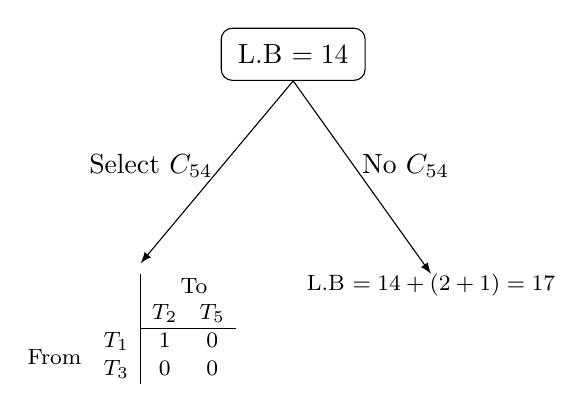
\begin{tikzpicture}[
                shift={(-0.35cm,0)},
                subroot/.style={rectangle, rounded corners, draw, inner sep=6pt, align=center},
                leaf/.style={anchor=north, inner sep=0pt, outer sep=0pt, draw=none},
            ]
            \node[subroot] (subrootC54) {L.B $= 14$};
            \node[leaf, align=center] (c54L) at ($ (subrootC54.south) + (-2.05,-2.45) $) {%
                \footnotesize
                \renewcommand{\arraystretch}{1.06}%
                \setlength{\tabcolsep}{4pt}%
                \begin{tabular}{@{}ll|cc@{\hspace{4pt}}l@{}}
                \multicolumn{2}{@{}r|}{} & \multicolumn{2}{c@{}}{To} & \\[-0.15ex]
                \multicolumn{2}{@{}r|}{} & $T_2$ & $T_5$ & \\
                \cline{3-4}
                \multirow{2}{*}[-1pt]{\raisebox{0pt}[0pt][0pt]{From}} & $T_1$ & 1 & 0 & \\
                & $T_3$ & 0 & 0 & \\
                \end{tabular}%
            };
            \node[leaf] (c54R) at ($ (subrootC54.south) + (1.75,-2.45) $) {\footnotesize L.B $= 14 + (2 + 1) = 17$};
            \draw[-latex, shorten >=5pt] (subrootC54.south) -- node[midway, auto=right, inner sep=0pt, outer sep=0pt] {Select $C_{54}$} (c54L.north);
            \draw[-latex] (subrootC54.south) -- node[midway, auto=left, inner sep=0pt, outer sep=0pt] {No $C_{54}$} (c54R.north);
            \end{tikzpicture} \\
            $\Rightarrow$ \text{Not using $C_{15}$ results in a lower bound of $15$.} \\
            $\Rightarrow$ \text{Must use $C_{15}$ and $C_{32}$} \vspace{0.5em} \\ 
            $\Rightarrow$ \boxed{\text{The toy sequence $T_{1}-T_{5}-T_{4}-T_{3}-T_{2}-T_{1}$ with cost $14$.}}
            \end{center} \vspace{0.5em} 
    \noindent\textbf{7.} \text{(a)} \begin{tabular}[t]{l}
        Use the approximate alogrithm to find approximate traveling salesperson tours \\
        for the cost matrix in Exercise 5 (use just entries above the main diagonal). \\ \\
        {\centering
            \renewcommand{\arraystretch}{1.25}%
            \setlength{\tabcolsep}{12pt}%
            \begin{tabular}{@{}ll|ccccc@{\hspace{10pt}}l@{}}
            \multicolumn{2}{@{}r|}{} & \multicolumn{5}{c@{}}{To} & \\[-0.2ex]
            \multicolumn{2}{@{}r|}{} & $T_1$ & $T_2$ & $T_3$ & $T_4$ & $T_5$ & \\
            \cline{3-7}
            \multirow{5}{*}[-2pt]{\raisebox{0pt}[0pt][0pt]{From}} & $T_1$ & $\infty$ & 3 & 2 & 4 & 3  \\
            & $T_2$ & 3 & $\infty$ & 4 & 5 & 5 &  \\
            & $T_3$ & 2 & 4 & $\infty$ & 4 & 4 & \\
            & $T_4$ & 4 & 5 & 4 & $\infty$ & 6 & \\
            & $T_5$ & 3 & 5 & 4 & 6 & $\infty$ &  \\
            \end{tabular}\par
        } \\ \\ %
        \text{- Select $T_{1}$}
    \end{tabular}
    \begin{center}
        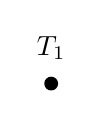
\begin{tikzpicture}[baseline=-3pt]
            \coordinate (T1) at (0,0);
            \fill[black] (T1) circle (2.5pt);
            \node[above=5pt] at (T1) {$T_1$};
        \end{tikzpicture}
    \end{center}
    \indent \indent \indent \begin{tabular}[t]{l}
        \text{- Add $T_{3}$ to the circuit $C$ ($T_1$ is 2 units away from $T_3$)}
    \end{tabular}
    \begin{center}
        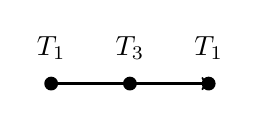
\begin{tikzpicture}[baseline=-3pt]
            \coordinate (T1) at (0,0);
            \fill[black] (T1) circle (2.5pt);
            \node[above=5pt] at (T1) {$T_1$};

            \coordinate (T0) at (2,0);
            \fill[black] (T0) circle (2.5pt);
            \node[above=5pt] at (T0) {$T_1$};

            \coordinate (T3) at (1,0);
            \fill[black] (T3) circle (2.5pt);
            \node[above=5pt] at (T3) {$T_3$};
            \draw[->, thick] (T1) -- (T3) -- (T0);
        \end{tikzpicture}
    \end{center}
    \indent \indent \indent \begin{tabular}[t]{l}
        \text{- Add $T_{2}$ to $C$ ($T_2$ is 3 units away from $T_1$)}
    \end{tabular}
    \begin{center}
        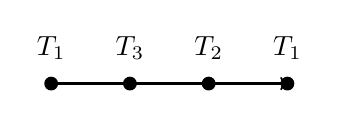
\begin{tikzpicture}[baseline=-3pt]
            \coordinate (T1) at (0,0);
            \fill[black] (T1) circle (2.5pt);
            \node[above=5pt] at (T1) {$T_1$};

            \coordinate (T0) at (3,0);
            \fill[black] (T0) circle (2.5pt);
            \node[above=5pt] at (T0) {$T_1$};

            \coordinate (T3) at (1,0);
            \fill[black] (T3) circle (2.5pt);
            \node[above=5pt] at (T3) {$T_3$};

            \coordinate (T2) at (2,0);
            \fill[black] (T2) circle (2.5pt);
            \node[above=5pt] at (T2) {$T_2$};

            \draw[->, thick] (T1) -- (T3) -- (T2) -- (T0);
        \end{tikzpicture}
    \end{center}
    \indent \indent \indent \begin{tabular}[t]{l}
        \text{- Add $T_{5}$ to $C$ ($T_5$ is 3 units away from $T_1$)}
    \end{tabular}
    \begin{center}
        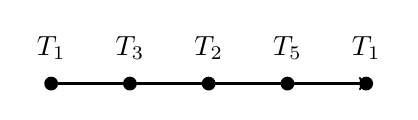
\begin{tikzpicture}[baseline=-3pt]
            \coordinate (T1) at (0,0);
            \fill[black] (T1) circle (2.5pt);
            \node[above=5pt] at (T1) {$T_1$};

            \coordinate (T0) at (4,0);
            \fill[black] (T0) circle (2.5pt);
            \node[above=5pt] at (T0) {$T_1$};

            \coordinate (T3) at (1,0);
            \fill[black] (T3) circle (2.5pt);
            \node[above=5pt] at (T3) {$T_3$};

            \coordinate (T2) at (2,0);
            \fill[black] (T2) circle (2.5pt);
            \node[above=5pt] at (T2) {$T_2$};

            \coordinate (T5) at (3,0);
            \fill[black] (T5) circle (2.5pt);
            \node[above=5pt] at (T5) {$T_5$};
            \draw[->, thick] (T1) -- (T3) -- (T2) -- (T5)-- (T0);
        \end{tikzpicture}
    \end{center}
    \indent \indent \indent \begin{tabular}[t]{l}
        \text{- Add $T_{4}$ to $C$ ($T_4$ is 3 units away from $T_3$)}
    \end{tabular}
    \begin{center}
        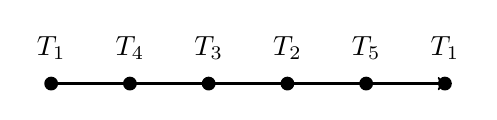
\begin{tikzpicture}[baseline=-3pt]
            \coordinate (T1) at (0,0);
            \fill[black] (T1) circle (2.5pt);
            \node[above=5pt] at (T1) {$T_1$};

            \coordinate (T0) at (5,0);
            \fill[black] (T0) circle (2.5pt);
            \node[above=5pt] at (T0) {$T_1$};

            \coordinate (T3) at (2,0);
            \fill[black] (T3) circle (2.5pt);
            \node[above=5pt] at (T3) {$T_3$};

            \coordinate (T2) at (3,0);
            \fill[black] (T2) circle (2.5pt);
            \node[above=5pt] at (T2) {$T_2$};

            \coordinate (T5) at (4,0);
            \fill[black] (T5) circle (2.5pt);
            \node[above=5pt] at (T5) {$T_5$};

            \coordinate (T4) at (1,0);
            \fill[black] (T4) circle (2.5pt);
            \node[above=5pt] at (T4) {$T_4$};

            \draw[->, thick] (T1) -- (T4) -- (T3) -- (T2) -- (T5) -- (T0);
        \end{tikzpicture}
    \end{center}
\end{document}